\chapter{Jäähdytysalgoritmin soveltaminen kiekko-ongelmaan}
\label{cha:algoritmin_soveltaminen}

\section{Kiekko-ongelman muotoilu optimointiongelmana}
\label{sec:kiekko_ongelman_muotoilu_optimointiongelmana}

Oletetaan että kuva $A_\text{data}$ esittää edellisessä luvussa esitellyn mallin mukaisesti yhtä ympyräkiekkoa $w_0 = (x_0, y_0, r_0)$,
jonka parametrit ajatellaan tuntemattomiksi vakioiksi jotka halutaan selvittää.
Tämä yhden kiekon kiekko-ongelma voidaan ajatella määritelmän~\ref{maar:globaali_optimointiongelma} mukaisena globaalina diskreettinä optimointiongelmana,
jossa pyritään löytämään muuttujille $x, y, r$ arvot jotka \emph{minimoivat} niitä vastaavan havaintomallin kuvan $A_\text{havaittu}$ eron $A_{\text{data}}$:aan.
Monen kiekon tapauksessa vastaavasti pyritään minimoimaan jokaista kuvan $A_{\text{data}}$ esittämän kiekkokokoelman $W = (w_0, \dots, w_k)$ kiekkoa vastaavat parametrit.

Jos kuvien resoluution ajatellaan olevan tarpeeksi suuri,
kiekko-ongelmaa olisi myös perusteltua mallintaa \emph{jatkuvan} optimoinnin tehtävänä eikä kombinatorisena optimointiongelmana,
johon tässä tutkielmassa kuvattu ''klassinen'' SA soveltuu,
Esimerkiksi \textcite{recipes07} ehdottavat jäähdytysmenetelmän jatkuvassa tapauksessa hieman hienostuneempaa menetelmää uuden tilan $s_j$ valitsemiseen.
Käytännössä diskreetti algoritmi kuitenkin toimii kiekko-ongelmaan,
ja joka tapauksessa teoreettisesti jatkuva parametriavaruus on diskreetti laskentatarkkuuden puitteissa.

Muotoillaan $k$ kiekon ongelma äärelliselle $k \in \Natural$ (josta yhden kiekon ongelma saadaan erikoistapauksena $k=1$) optimointiongelmana,
johon sovelletaan jäähdytysalgoritmia.
Määritellään algoritmin tilat ja valitaan sopiva energiafunktio ja jäähdytysstrategia.

\begin{maar}
    Yhden kiekon tapauksessa sanomme että kiekon $w_i$ määrittävät parametrit $x_i, y_i, r_i$ muodostavat yhdessä jäähdytysalgoritmin tilan (tai ratkaisuehdokkaan tai konfiguraation) $s_i$,
    \begin{equation}
        s_i = (x_i, y_i, r_i) \in m \times n \times \R
    \end{equation}
    Vastaavasti monen kiekon ongelmassa kun kiekkojen määrä $k$ on tunnettu, systeemin tila $s_i$ on kokoelma kiekkoja $W$ eli ne määritteleviä parametrivektoreita,
    \begin{align}
        \label{eq:tila_monta_kiekkoa}
        s_i &= \{s_{i, 1}, \dots, s_{i, k}\} \\
            &= \{(x_{i,1}, y_{i,1}, r_{i,1}), \dots, (x_{i,k}, y_{i,k}, r_{i,k})\},
    \end{align}
    jotka voidaan tarpeen vaatiessa esittää esimerkiksi matriisina
    \begin{equation}
        s_i =
        \begin{bmatrix}
            (x_{i,1}, y_{i,1}, r_{i,1}) & \dots & (x_{i,k}, y_{i,k}, r_{i,k})
        \end{bmatrix}.
    \end{equation}
\end{maar}

\section{Energiafunktio}
\label{sec:energiafunktio}

Määritellään seuraavaksi edellisessä luvussa~\customref{cha:kuvamalli_ja_aineisto} esitellyn havaintomallin~\eqref{eq:kuvamalli}
\begin{equation*}
    \tag{\ref{eq:kuvamalli}}
    A_\text{havaittu} = P \ast A_W + E
\end{equation*}
pohjalta sopiva optimoitava energiafunktio.

\subsection{Naiivi energiafunktio}
\label{sub:naiivi_energiafunktio}

Kuten aiemminkin, merkitään kuvadatamatriisia $A_{\text{data}}$, ja parametrien $x, y, r$ määräämää ympyrää $w$ esittävä matriisia $A_{x, y, r} = A_w$.
Mallin~\eqref{eq:kuvamalli} ytimellä konvolvoitu kuvamatriisi on $P \ast A_w$,
jonka avulla voidaan määritellä eräs yksinkertainen energiafunktio:

Energiafunktio $E_\text{naiivi}$ on $P \ast A_w$:n 'pikselikohtainen' ero matriisiin $A_{\text{data}}$,
eli erotuksen $A_{\text{data}} - P \ast A_w$ alkioittainen euklidisen normin neliö
\begin{equation}
    E_\text{naiivi}(s) = E_\text{naiivi}(x, y, r) = \sum_i \sum_j \left(A_{\text{data}}(i, j) - P \ast A_w(i, j)\right)^2.
\end{equation}

Luvussa~\ref{cha:kuvamalli_ja_aineisto} määriteltiin myös malli usean $k$ kiekon kokoelmaa $W = \left\{w_1, \dots, w_k\right\}$ vastaavalle kuvalle $A_W$, ja
$E_\text{naiivi}$ yleistyy suoraan kokoelmalle $W$ kun tila $s$ yleistetään monelle kiekolla kuten yllä yhtälössä~\eqref{eq:tila_monta_kiekkoa}:
\begin{equation}
    E_\text{naiivi}(s) = \sum_i \sum_j \left(A_{\text{data}}(i, j) - P \ast A_W(i, j)\right)^2.
\end{equation}

Suoraan nähdään, että energiafunktion kannalta parempi on sellainen tila $s$, jonka parametrit ovat lähellä käyttämämme mallin mukaisia ''todellisia'' kiekkoparametreja $W = s_\text{opt}$,
ja vastaavasti tilat $s'$, joiden kiekot kaukana $A_\text{data}$ todellisista kiekoista ovat energiafunktion $E_\text{naiivi}$ huonompia.

Ilman datan kohinaa ja mallin epätarkkuutta ($P \not = P_\text{data}$) edellä määritelty energiafunktio saavuttaisi globaalin minimin $E_\text{naiivi}(s_\text{opt}) = 0$.
Virheilähteiden vuoksi tämä ei ole luultavasti täysin mahdollista, mutta voidaan olettaa että suurella todennäköisyydellä energiafunktio on tässä suhteessa edelleen hyvä kohinasta ja epätarkasta sumennosmallista huolimatta.

\subsection{Energiamaasto}
\label{sub:energiamaasto}

Tarkastellaan seuraavaksi energiafunktion $E_\text{naiivi}$ 'energiamaastoa' eli sen parametriavaruudessaan saamia arvoja ( \emph{energy landscape} \cite{salamonetal}):

Ensinnäkin $E_\text{naiivi}$ ei erota toisistaan kahta eri tilavektoria $s$ ja $s'$, mikäli niitä vastaavat ympyrät eivät osu päällekkäin minkään $A_{\text{data}}$:n ympyräobjektin kanssa.
Toisin sanoen, vaikka toinen tilavektori $s$ olisi paljon lähempänä optimia kuin $s'$.
(Ks.~kuva~n.)
Käytännössä algoritmi ei pysty parempaan kuin satunnaisiin arvauksiin kunnes tilakandidaattien $s_i$ satunnaiskulku osuu sellaiseen kandidaattiin, jota vastaava ympyrä on osittain $A_{\text{data}}$:n tavoiteympyrän päällä;
vasta tämän jälkeen energiafunktio pystyy mittaamaan uuden tilaehdokkaan $s_j$ paremmuutta suhteessa edelliseen $s_i$.

Hyvin pienillä ympyrän säteillä tehtävä muistuttaa yhtä enemmän sellaista optimointiongelmaa, jota \textcite{salamonetal} kutsuvat 'golf-reikäongelmaksi':
tasaisessa energiamaastossa on pieni alue, joka ei näy ympäröivässä energiamaastossa (ikään kuin golf-kentän reikä), jossa saavutetaan globaali minimi.
(Kuva~\ref{fig:golfholes}.)
Tälläisen yksittäisten, algoritmin näkökulmasta satunnaisten minimipisteiden löytämiseen on vaikea löytää satunnaishakua parempaa strategiaa.
SA-algoritmi pyrkii vastaamaan tähän korkean lämpötilan ratkaisujen satunnaisuudella:
sopivalla jäähdytysskenaariolla ratkaisu löydetään vielä lämpötilan $t$ ollessa korkea ja suuri osa parametriavaruudesta on satunnaiskulun tavoitettavissa,
mikä on kuitenkin kiekkojen säteiden kutistuessa pistemäisiksi yhä vaikeampaa.

Toiseksi kuvan reunat muodostavat $E_\text{naiivi}$:n suhteen \emph{lokaalin} minimin (ks.~kuva~\ref{fig:golfhole3}),
samoin tilavektorit $s$ joissa kiekkokandidaatit asettuvat osittain päällekkäin pyrkien kattamaan esimerkiksi vain yhden suurempia $A_\text{data}$:n kiekon mahdollisimmaan tarkkaan (kuva~\ref{fig:localmins2}).

\subsection{Paranneltu monen kiekon energiafunktio}
\label{sub:paranneltu_monen_kiekon_energiafunktio}

Kiekkojen lukumäärän ja ratkaisuavaruuden $\Omega$ ulottuvuuksien määrän kasvaessa päällekkäisten kandidaattien lokaalien minimien määrä moninkertaistuu nopeasti
ja vaikeuttaa optimaalisen ratkaisun $s_\text{opt}$ löytämistä. (Kuva~\ref{fig:localmins2}.)
Tämän vuoksi määritellään myös paranneltu energiafunktio $E_\text{par}$,
joka rankaisee päällekkäisistä kandidaattikiekoista.
(Tutkituissa aineistoissa $A_{\text{data}}$:ssa ei ole päällekkäisiä kiekkoja.)

Määritellään ensin kuvamatriisin $A$ intensiteettikäänteiskuva
\begin{equation*}
    A' = 1 - A =
        \begin{cases}
            A(i,j)' &= 0, \text{ jos } A(i,j) = 1\\
            A(i,j)' &= 1, \text{ jos } A(i,j) = 0
        \end{cases}
\end{equation*}
ja reaalilukuarvoinen apumatriisi $\Delta A \in \R^{m\times n}$,
\begin{equation}
    \Delta A = 1 - \left( A_{w_1}' + \dots + A_{w_k}' \right),
\end{equation}
missä $1$ on $A$:n kokoinen ykkösmatriisi ja yhteenlasku- ja erotus tavallisia matriisioperaatiota.
Matriisin \Delta A avulla voidaan nyt määritellä paranneltu energiafunktio
\begin{equation}
    \label{eq:paranneltu_energiafunktio}
    E_\text{par}(s) = E_\text{par}(w_1, \dots, w_k) = \sum_i \sum_j \left(  A_{\text{data}}(i,j) - P \ast \Delta A(i,j) \right)^2.
\end{equation}

Nähdään, että jos kiekot $w_1, \dots, w_k$ ovat erillisiä, pätee $1 - \left(A_{w_1}' + \dots + A_{w_k}'\right) = A_{w_1, \dots, w_k} = A_W$,
ja $E_\text{par}$ saisi kyseisillä parametrin arvoilla saman arvon kuin $E_\text{naiivi}$.
Sellaisten pikseleiden $(i,j)$ joiden kohdalla useampi kiekko osuu päällekkäin,
apumatriisin pikselit $\Delta A(i,j)$ ovat negatiivisia, toisin kuin vastaavassa kuvamatriisissa $A_W$,
jonka elementeille pätee
\begin{equation*}
    A_W(i,j) \in [0, 1].
\end{equation*}
Näin ollen yhtälön~\eqref{eq:paranneltu_energiafunktio} energiafunktio $E_\text{sov}$ saa päällekkäisten kiekkojen kohdalla suuremman arvon kuin $E_\text{naiivi}$, sillä
\begin{equation*}
    A_\text{data}(i,j) - P \ast \Delta A (i,j) > A_\text{data}(i,j) - P \ast A_W(i,j).
\end{equation*}
Käytännön esimerkki kuvassa~\ref{fig:localmins}.


\begin{figure}[p]
    \centering
    \hspace{-1em}
    \begin{subfigure}[b]{0.3\textwidth}
        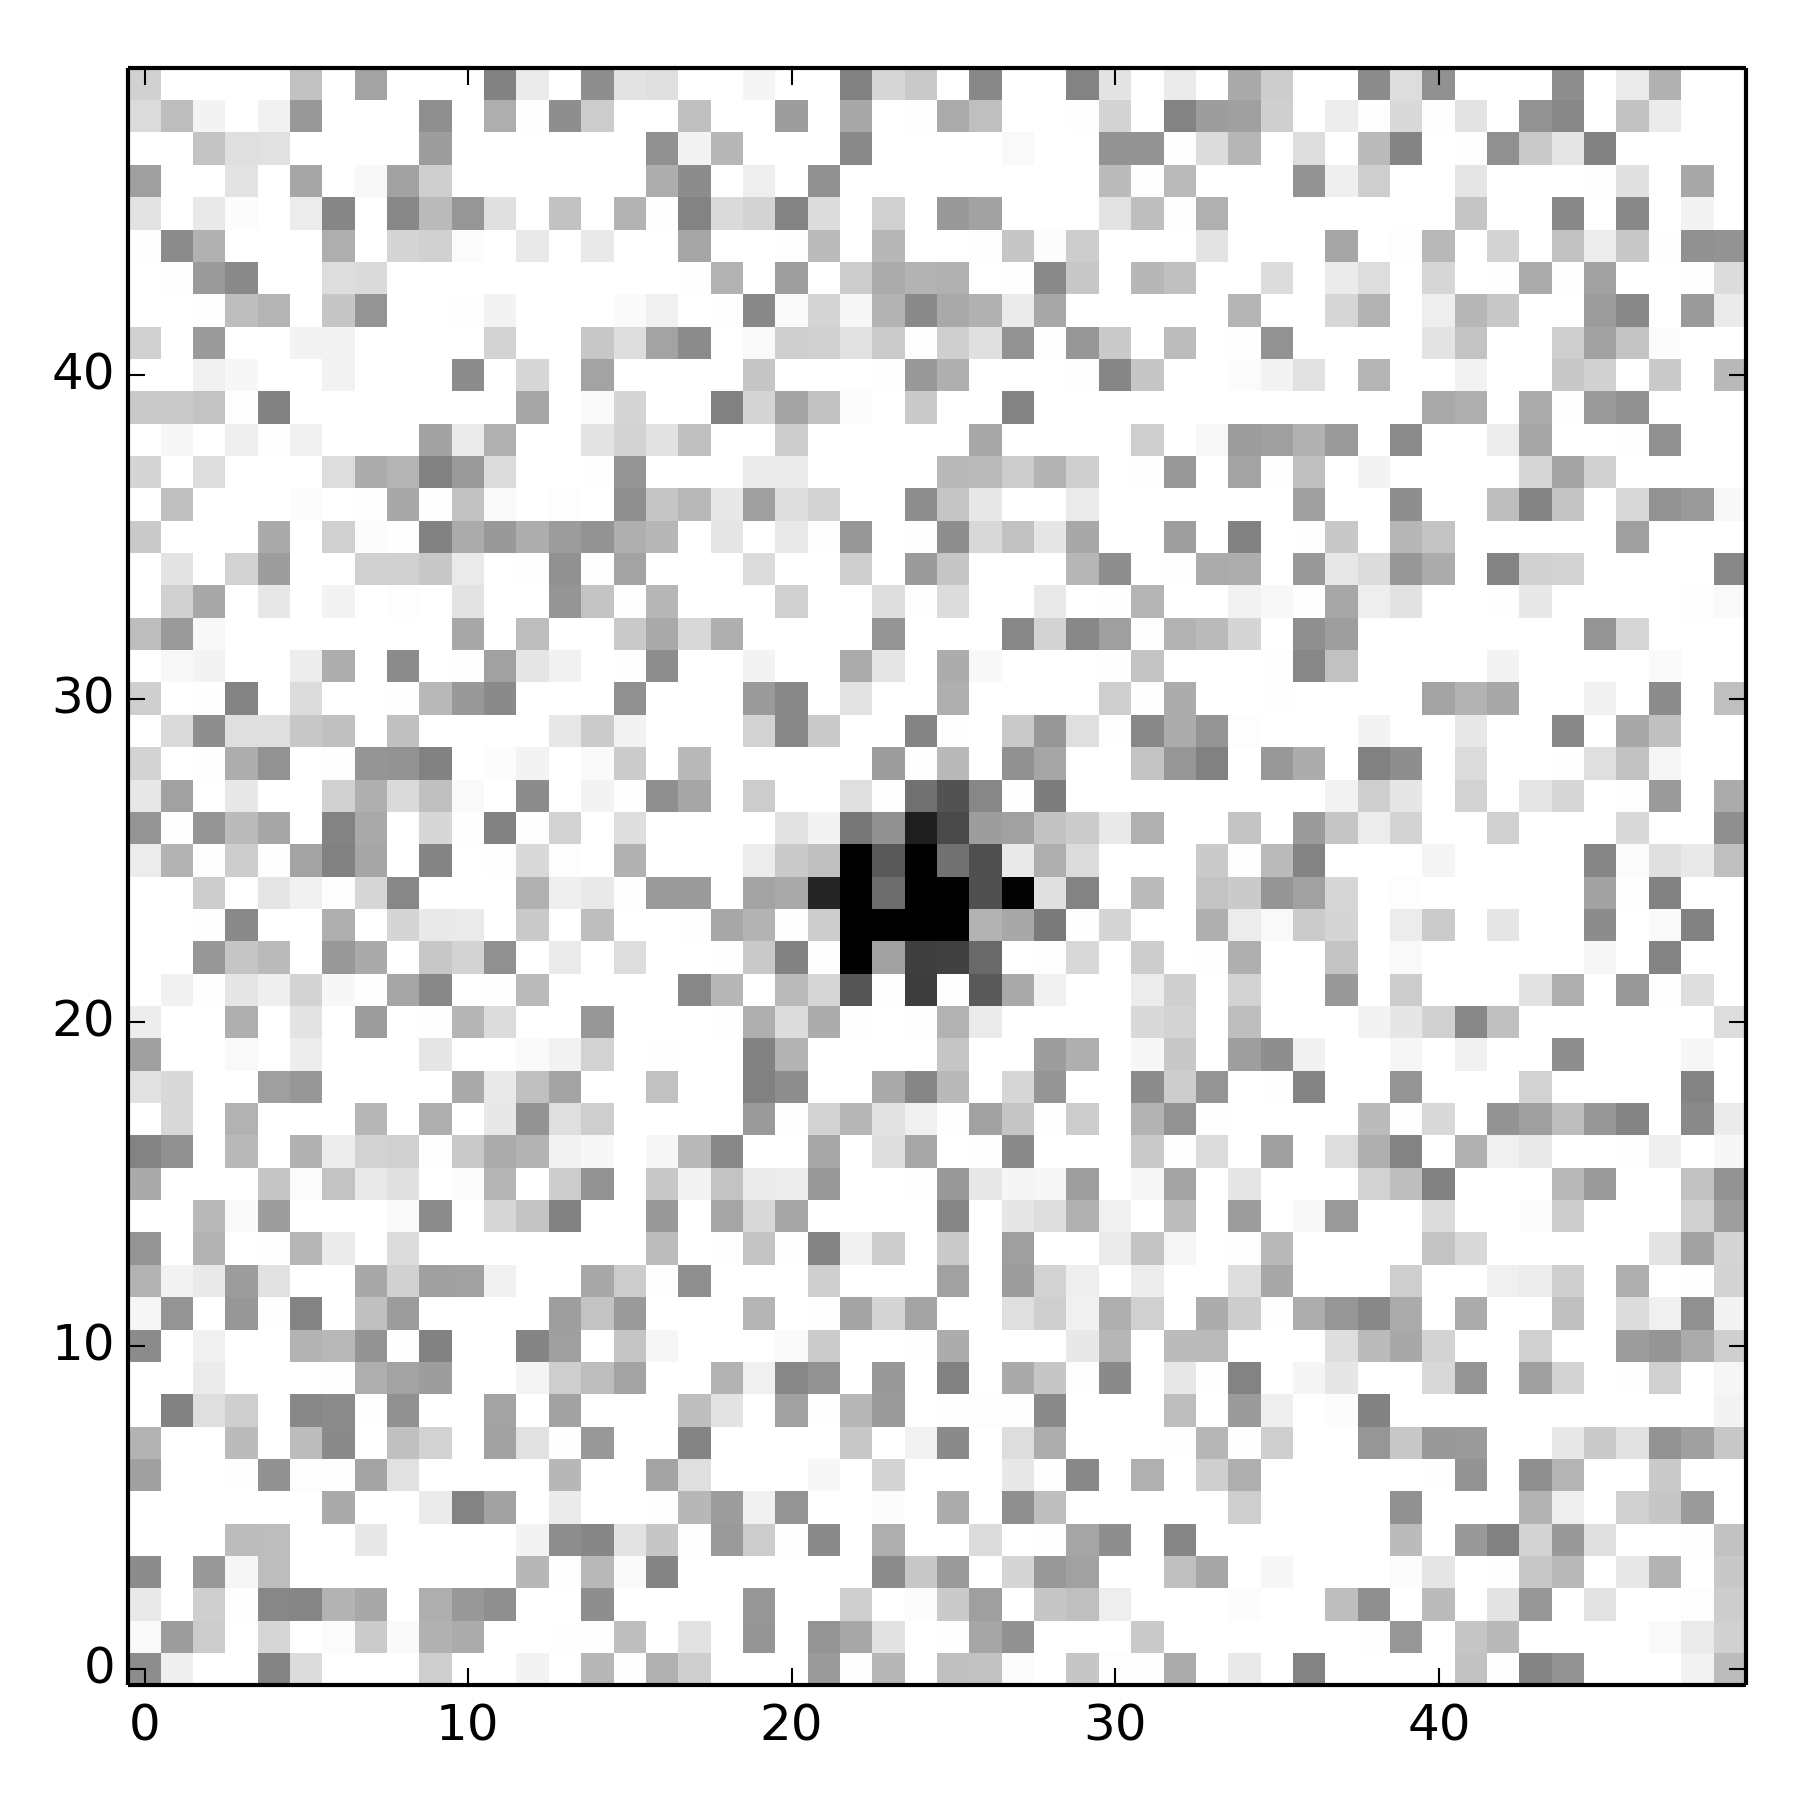
\includegraphics[width=\textwidth]{figures/golfholedata.png}
        \caption{$A_\text{data}$, $r=3$.
            \label{fig:golfhole_data}
        }
    \end{subfigure}

    \begin{subfigure}[b]{0.7\textwidth}
            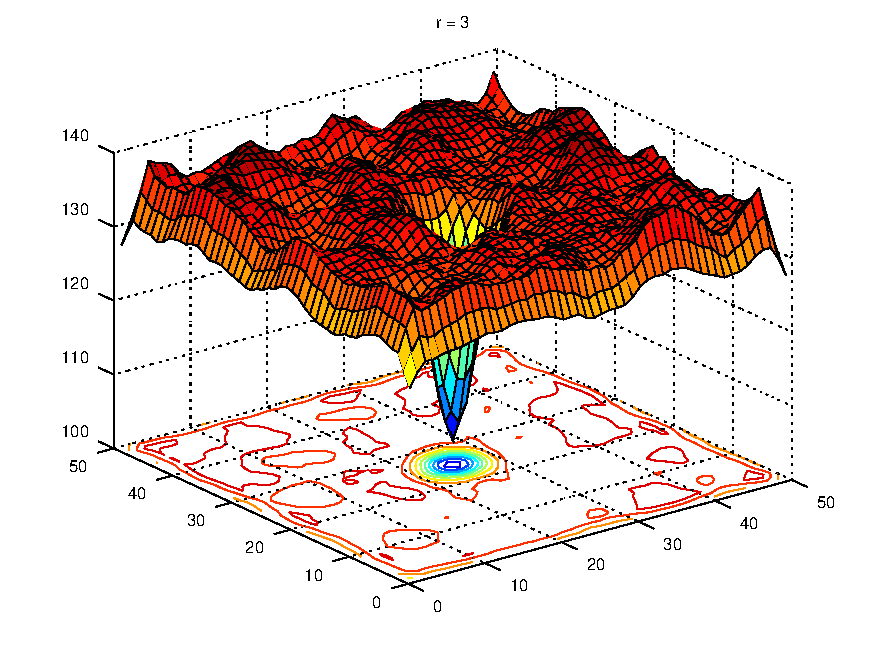
\includegraphics[width=\textwidth]{figures/golfhole2.pdf}
        \caption{Kiinteä $r=3$. 
            \label{fig:golfhole2}
        }
    \end{subfigure}

    \begin{subfigure}[b]{0.7\textwidth}
            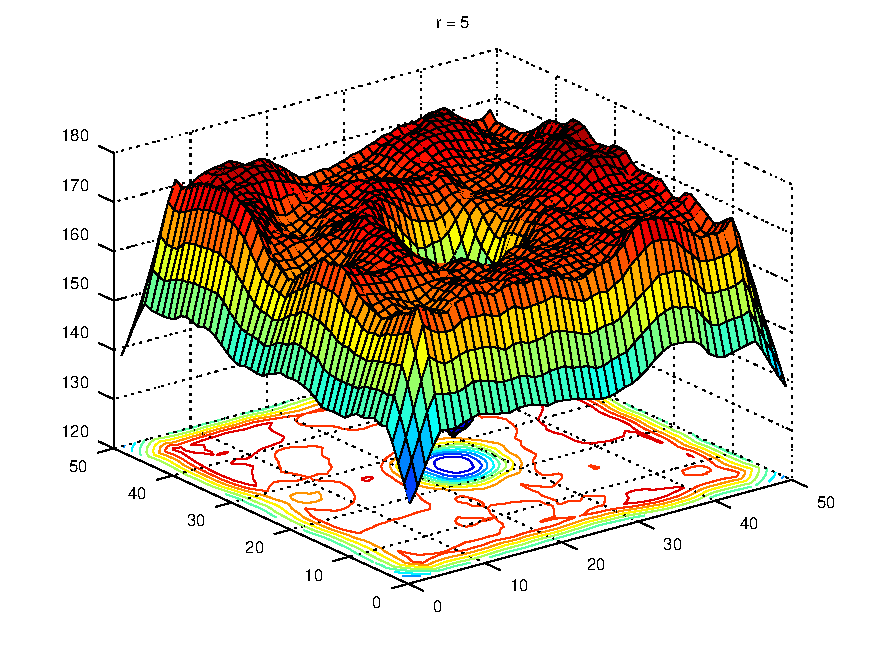
\includegraphics[width=\textwidth]{figures/golfhole3.pdf}
        \caption{Kiinteä $r=5$.
            \label{fig:golfhole3}
        }
    \end{subfigure}
    \caption{Energiafunktion $E_\text{naiivi}$ energiamaasto $xy$-avaruudessa.
        Energiamaasto on $xy$-ulottuvuudessa golf-reikämäinen (kuva~\ref{fig:golfhole2}), mutta $r$-ulottuvuudessa globaalin minimin 'kuoppa' näkyy alati laajemmalla alueella kun $r$ kasvaa.
        Huomaa myös reunojen lokaalit minimit.
        \label{fig:golfholes}}
\end{figure}


\begin{figure}[p]
    \centering
    \begin{subfigure}[b]{0.3\textwidth}
        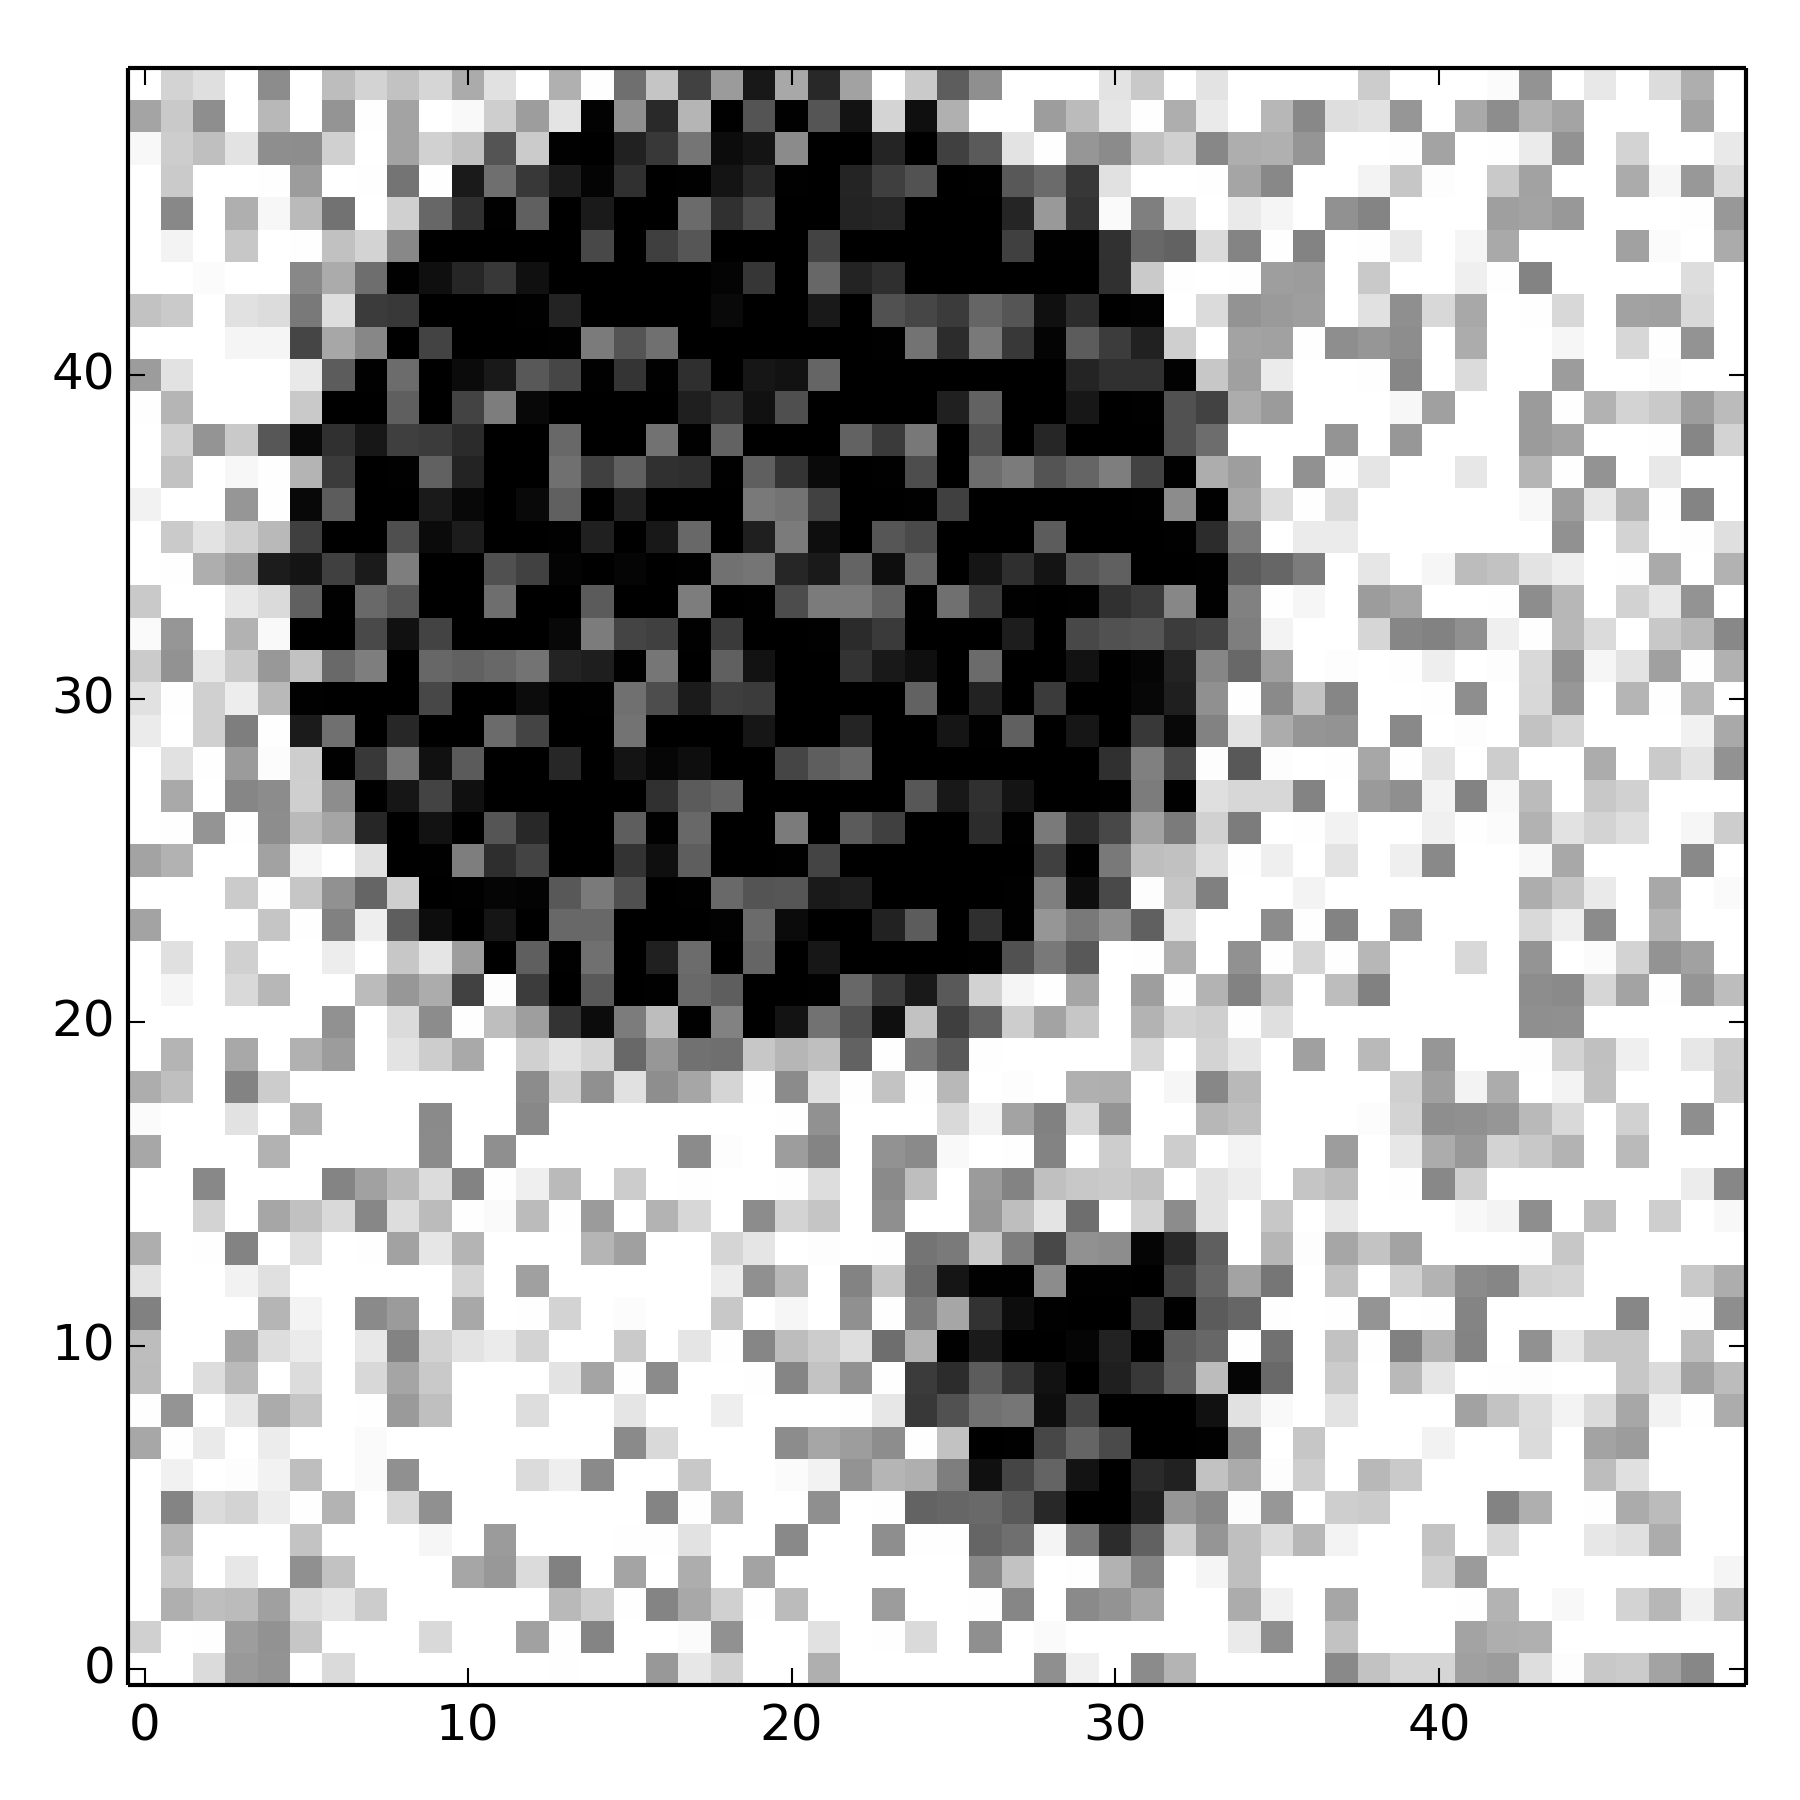
\includegraphics[width=\textwidth]{figures/localmindata.png}
        \caption{$A_\text{data}$. $(x_i,y_i,r_i) = (35, 20, 15), (10, 30, 5)$.
            \label{fig:localmin_data}
        }
    \end{subfigure}

    \begin{subfigure}[b]{0.7\textwidth}
            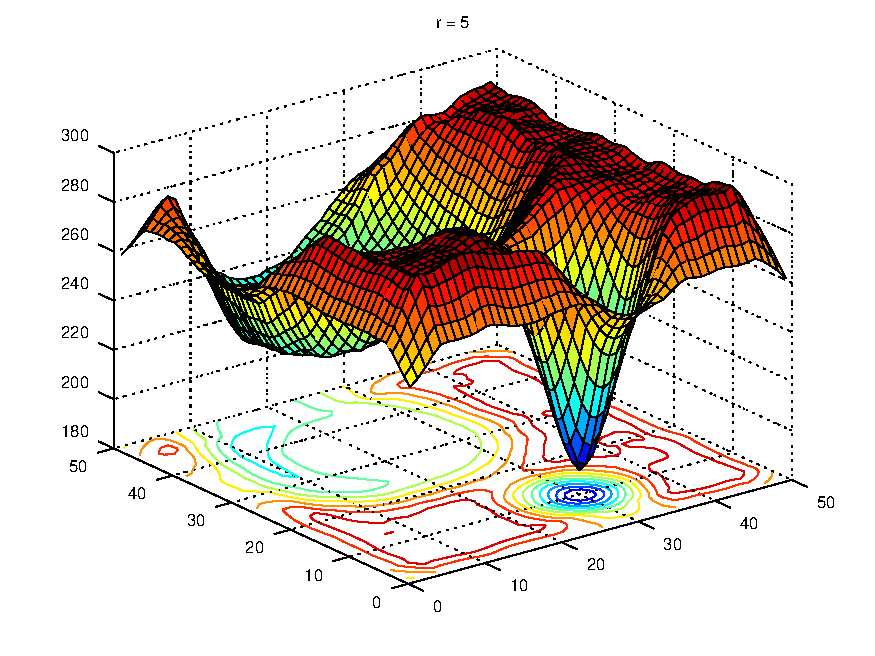
\includegraphics[width=\textwidth]{figures/localmins2.pdf}
        \caption{
            $E_\text{naiivi}$.
            \label{fig:localmins2}
        }
    \end{subfigure}

    \begin{subfigure}[b]{0.7\textwidth}
            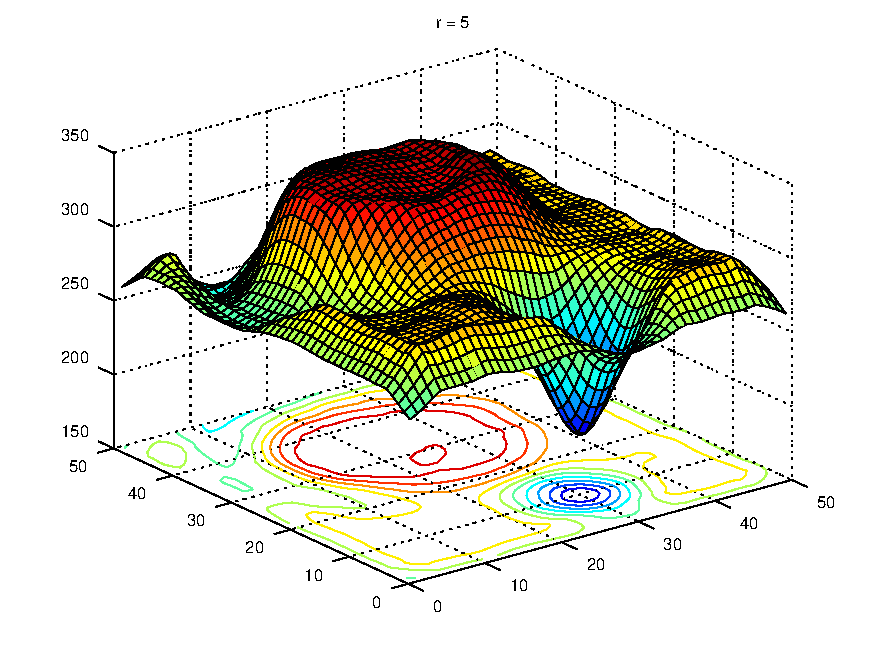
\includegraphics[width=\textwidth]{figures/localmins4.pdf}
        \caption{$E_\text{sov}$
            \label{fig:localmins4}
        }
    \end{subfigure}
    \caption{Energiafunktioiden $E_\text{naiivi}$ ja $E_\text{sov}$ arvoja toisen kiekon $x_2 y_2$-avaruudessa kun toisen kiekon säde $r_2=5$ ja ensimmäisen kiekon parametrit pidetään vakioina $(x_1, y_1, r_1) = (34, 22, 14)$.
        $E_\text{sov}$ rankaisee tiloista, joissa toinen parametrikiekko on ensimmäisen päällä.
        \label{fig:localmins}}
\end{figure}


\section{Siirtymät}
\label{sec:siirtymat}

Yksinkertaisin tapa toteuttaa jäähdytysalgoritmin 'pieni satunnainen siirtymä' olisi satunnaisesti valita jokin muuttujista $x, y, r$ ja lisätä tai vähentää siitä jokin kiinteä, pieni luku $\delta > 0$.
Käytännössä näin saataisiin jatkuvan parametriavaruuden $\Omega$ diskretisointi.
Tällöin kuitenkin joko menetettäisiin ratkaisutarkkuutta (jos $\delta$ on suuri) tai pienellä vakion arvolla $\delta \approx \text{pikseli}$ siirtymät olisivat liian pieniä jotta lagoritmi kävisi ratkaisuavaruutta läpi tehokkaasti.

Tämän vuoksi käytetään seuraavaa menetelmää siirtymien generointiin:
Valitaan satunnainen kiekko, jonka parametrit ovat $(x, y, r)$.
Uusi piste $(x',y',r')$ valitaan $(x, y, r)$ -keskisen 'ellipsoidin' sisältä parametriavaruudessa $\Omega$:
\begin{align}
    r' &= \delta \cdot r, \qquad \delta \sim U(-1, 1),\\
    (x', y') &= (x, y) + \delta \cdot (\cos(\phi), \sin(\phi)), \qquad \phi \in U(0, 2\pi).
\end{align}

Lisäksi rajoitetaan $x,y$-siirtymiä siten ettei kiekon keskipiste voi mennä kuva-alueen $A$ ulkopuolelle.
Vastaavasti estetään arvot $r < 1$ pikseli ($r = 0$ muodostaisi myös lokaalin minimin) ja $r >$ kuvan koko.


\section{Jäähdytysstrategia}
\label{sec:jaahdytysstrategia}


SA-algoritmin jäähdytysstrategian valitsemiseen yleisesti kirjallisuus (\cite{laarhoven}, \cite{salamonetal}, \cite{recipes07}) tarjoaa lukuisia hyvin erilaisia vaihtoehtoja.
Tässä tutkielmassa käytetään yksinkertaista eksponentiaalista jäähdytysstrategiaa.

\subsection{Lämpötilan laskeminen}
\label{sub:lampotilan_laskeminen}

Lämpötilaa homogeenilla ketjulla $k$ päivitetään yhtälön
\begin{equation}
    t_{k+1} = \alpha \cdot t_k, \qquad k = 0, 1, 2, \dots
\end{equation}
mukaisesti,
missä $\alpha$ on vakio $1 - \epsilon$ jollekin pienelle $\epsilon >0$.
(Käytännössä 'pienellä' tarkoitamme että kokeilemme luvussa~\ref{cha:tulokset} arvoja $\alpha = 0.90 \dots 0.99$.)

Markov-ketjun pituus kullakin kontrolliparametrin arvolla $t_k$ asetetaan vakioksi $L_k = 10$.


\subsection{Lämpötilan alkuarvo}
\label{sub:lampotilan_alkuarvo}

Kontrolliparametrin alkuarvo $t_0$ eli lähtölämpötila pyritään valitsemaan siten,
että lämpötilan ensimmäisillä arvoilla hyväksyttyjen tilamuutosten suhde kaikkiin yritettyihin  tilamuutoksiin  $q$ on lähellä yhtä, eli
\begin{equation}
    \label{eq:ratio}
    q_0 = \exp{-\mean{\Delta E} / t_0} \approx 1,
\end{equation}
missä $\mean{\Delta E}$ on 'keskimääräistä' satunnaista siirtymää vastaava energiafunktion muutos lämpötilassa $t_0$.
Toisaalta ei ole toivottavaa, että $t$ säilyy korkeana (ja $q \approx 1$) \emph{liian} pitkään, jolloin siitä ei enää hyötyä algoritmin toimivuuden kannalta ja simulointi korkeissa lämpötiloissa vie turhaan laskenta-aikaa.

Näin ollen kunkin algoritmin ajokerran alussa valitaan sopiva arvio saadaan yhtälön~\ref{eq:ratio} avulla:
\begin{align}
    \exp\left(-\mean{\Delta E} / t_0\right) &= q_0 \quad (\leq 1)\\
    t_0 &= -\frac{\mean{\Delta E}}{\log{q_0}}, \quad q_0 \leq 1,
\end{align}
missä keskimääräistä energiafunktion muutosta $\mean{\Delta E}$ kullakin $A_\text{data}$ arvioidaan simuloimalla muutamia jaksossa~\ref{sec:siirtymat} kuvailtuja siirtymiä.

\subsection{Loppukriteeri}
\label{sub:loppukriteeri}

Käytännön varotoimenpiteenä asetetaan maksimiraja kuinka monta iteraatiota algoritmia suoritetaan ($n = 1000$ homogeenia 10 iteraation Markov-ketjua).

Varsinaiseksi lopetuskriteeriksi asetamme kuitenkin sen lämpötilan, jossa Markov-ketjut alkavat toistua samankaltaisina,
eli uudet iteraatiot pienemmillä lämpötiloilla eivät enää vaikuta johtavan merkittävästi parempiin ratkaisuihin.
Käytännössä kelvolliseksi osoittautui katkaisuehto,
jossa algoritmin iteraatio $i$ jää viimeiseksi $i := i_\text{final}$, jos
\begin{equation}
    \frac{\sum_{j=0,\dots,3} q_{i-j}}{4} < 0.05.
\end{equation}




